\subsection{Opis języka}

Aplikacja potrafi wygenerować podstawowe elementy diagramu klas oraz diagramu przypadków użycia zdefiniowane w standardzie UML 2.0.

\subsubsection{Klasa}

Klasę definiuje się na podstawie prototypu \textbf{class}.\footnote{O prototypach będziem mowa w dalszej częsci}

    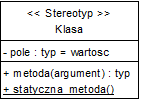
\includegraphics[width=\textwidth]{klasa}
Utworzony został obiekt o identyfikatorze \textbf{Klasa}. Na diagramie będzie to nazwą klasy. Można również nadać inną nazwę korzystając z klucza \textbf{name}(którego nie ma w przykładzie). Klucz \textbf{stereotype} pełni rolę stereotypów w języku UML. Przykładowa klasa posiada metodę(wraz ze statyczną) oraz pole. Na uwagę zasługuje okreslenie widocznosci metod i pól: +, -, ~, \#. Statyczne metody lub pola oznacza się poprzez \_.
Mając już zdefiniowaną klasę \textbf{Klasa} można utworzyć na jej podstawie następny obiekt, kopiując wszystkie ustawione wartosci kluczy z \textbf{Klasa}: \textbf{Klasa} NewObject.

\subsubsection{Relacja}

Relację okresla się na podstawie prototypu \textbf{relation}.

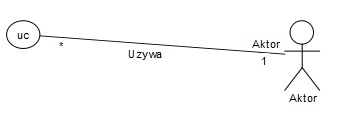
\includegraphics[width=\textwidth]{relacja}